\documentclass[11pt,a4paper]{article}

\usepackage[T1]{fontenc}
\usepackage[utf8]{inputenc}
\usepackage{lmodern}
\usepackage[a4paper,margin=2.4cm]{geometry}
\usepackage{microtype}
\usepackage{xcolor}
\usepackage{graphicx}
\usepackage{booktabs}
\usepackage{array}
\usepackage{tabularx}
\usepackage{longtable}
\usepackage{needspace}
\usepackage{amsmath}
\setlength{\LTpre}{4pt}\setlength{\LTpost}{6pt}
\renewcommand{\topfraction}{0.9}\renewcommand{\bottomfraction}{0.9}\renewcommand{\floatpagefraction}{0.75}
\usepackage{enumitem}
\usepackage{caption}
\usepackage{titlesec}
\usepackage{fancyhdr}
\usepackage{listings}
\usepackage{tikz}
\usetikzlibrary{arrows.meta,positioning}
\usepackage[hidelinks]{hyperref}

\definecolor{navy}{HTML}{1F3864}
\definecolor{blu}{HTML}{2A78D6}
\definecolor{ora}{HTML}{EB6834}

\titleformat{\section}{\Large\bfseries\color{navy}}{\thesection}{0.6em}{}
\titleformat{\subsection}{\large\bfseries\color{navy}}{\thesubsection}{0.6em}{}
\titlespacing*{\section}{0pt}{16pt}{6pt}
\titlespacing*{\subsection}{0pt}{12pt}{4pt}

\setlength{\parskip}{4pt}
\setlength{\parindent}{0pt}
\renewcommand{\arraystretch}{1.18}
\captionsetup{font=small,labelfont=bf,labelsep=period}
\setlist{itemsep=2pt,topsep=3pt}

\pagestyle{fancy}
\fancyhf{}
\renewcommand{\headrulewidth}{0.3pt}
\fancyhead[L]{\small DSA 8401 -- Applied Machine Learning}
\fancyhead[R]{\small ST-BMSE capstone report}
\fancyfoot[C]{\small\thepage}

\lstset{basicstyle=\ttfamily\small,backgroundcolor=\color{black!4},frame=none,breaklines=true,
  columns=fullflexible,xleftmargin=4pt,xrightmargin=4pt}

\newcommand{\code}[1]{\texttt{#1}}
\newcolumntype{R}{>{\raggedleft\arraybackslash}X}

\begin{document}

% ------------------------------------------------------------------ title
\begin{center}
  {\Huge\bfseries\color{navy} ST-BMSE\par}
  \vspace{4pt}
  {\LARGE\bfseries\color{navy} Forecasting County-Level Conflict\\ Escalation in Kenya\par}
  \vspace{10pt}
  {\large DSA 8401 Applied Machine Learning \textbullet{} Capstone Project Report\par}
  \vspace{4pt}
  {\large Esther Muthui (223932) \textbullet{} Strathmore University \textbullet{} November 2026\par}
\end{center}
\vspace{2pt}
\hrule height 0.8pt
\vspace{8pt}

\begin{abstract}\small\noindent
This report describes a reproducible machine-learning pipeline and model service that forecasts, for each of Kenya's 47
counties, the probability of conflict escalation \emph{next month}. A stacked ensemble of logistic regression, random
forest and XGBoost with empirical-Bayes Markov features, a calibrated meta-learner and a cost-sensitive alert threshold is
evaluated on an untouched 2022--2024 test period. It beats a persistence baseline (PR-AUC 0.61 vs.\ 0.50; paired
difference $+0.11$, 95\% CI $0.06$--$0.16$), but it does \emph{not} beat a single random forest, and the tuned alert
threshold flags almost every county. A leakage audit shows that same-month features give PR-AUC 0.97, which is a
nowcast rather than a forecast. The data are synthetic, built to the proposal's county-month design, so the results
demonstrate the method and should not be read as evidence about real conflict in Kenya; real ACLED and KNBS data are the planned next stage.
\end{abstract}

% ------------------------------------------------------------------ 1
\section{Problem framing}
\textbf{Task.} For each county, estimate the probability that it \emph{escalates in the next month}, using only
information known at the end of the current month. The output is a calibrated probability and an alert flag.

\textbf{Why it matters.} Early-warning practice relies largely on qualitative field reports, which are slow to compile and
hard to compare across counties. A ranked, calibrated county list lets analysts decide where to look first. The system is
decision support for a human reviewer, not an automated decision-maker.

\textbf{Unequal error costs.} A missed escalation can cost lives; a false alarm costs analyst time. The alert threshold
therefore minimises expected cost,
\begin{equation}
  \tau^\star=\arg\min_{\tau}\;\big[\,C_{FN}\,FN(\tau)+C_{FP}\,FP(\tau)\,\big],\qquad C_{FN}:C_{FP}=5:1,
\end{equation}
chosen on validation data. The 5:1 ratio is an \emph{assumption} of this project, not an elicited value.

% ------------------------------------------------------------------ 2
\section{Data and the complications built into the evaluation}
\textbf{Data.} \code{kenya\_conflict\_monthly.csv} has 5{,}640 rows (47 counties $\times$ 120 months, January 2015 to
December 2024), 13 columns, no missing values and no duplicate keys. The label \code{Conflict\_Escalation} is binary, with an
overall rate of 27.7\%.

\textbf{The data are synthetic.} They are simulated county-month records, not observed ACLED events~\cite{raleigh2010} or KNBS statistics.
They follow the proposal's design: 47 counties, monthly, January 2015 to December 2024, with 2022--2024 held out as the test period.
They carry the indicators the proposal's approach needs (conflict type, social unrest, economic volatility, diplomatic tension, security response time and sentiment)
plus a binary next-step escalation label. The proposal's plan to use ACLED events and KNBS indicators is the \emph{next stage}: the pipeline validates and consumes a fixed
county-month schema, so real data aggregated to that schema can replace the synthetic file.

Because the data are synthetic, the results show how the method behaves on data with this structure. They are not evidence about real conflict in Kenya,
and the proposal's data-quality plan (missing events, reporting changes, geocoding errors) is not exercised, since synthetic data are complete by construction.

\textbf{Complications that make the evaluation realistic.} The capstone brief asks for these explicitly.
\begin{enumerate}
  \item \textbf{Strict temporal protocol.} Train on targets up to 2019; tune the meta-learner and threshold on 2020--2021; report once on 2022--2024. No shuffling and no random $k$-fold.
  \item \textbf{Prior shift.} The escalation rate is 20.3\% in training, 23.7\% in validation and \textbf{42.9\% in the test period} (Figure~\ref{fig:drift}).
  \item \textbf{A leakage trap in the columns.} Several features describe the same month as the label (Section~\ref{sec:leak}). Preventing this kind of leakage is a core theme of the course text~\cite{serrano2026}.
  \item \textbf{No extra noise was injected.} The synthetic data are complete by construction and I added no missingness or label noise, so these complications come from the evaluation design and the data's own shift, not from injected problems.
\end{enumerate}
The proposal expected escalation to be ``relatively infrequent''. At 28\% overall and 43\% in the test period it is not,
so class imbalance is a minor issue on this file.

\begin{figure}[!htbp]
  \centering
  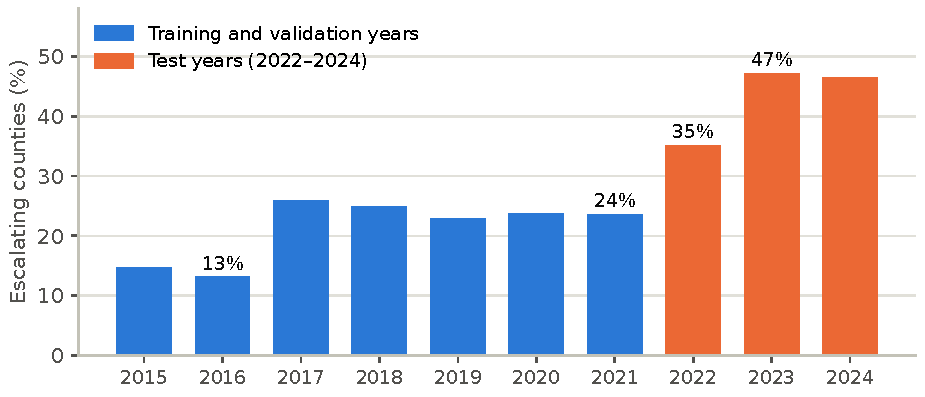
\includegraphics[width=0.92\linewidth]{figures/fig_drift.pdf}
  \caption{Share of counties escalating, by year. The base rate more than doubles between the training years and the test years.}
  \label{fig:drift}
\end{figure}

% ------------------------------------------------------------------ 3
\section{Pipeline}
The pipeline is scripted end to end (\code{python run\_pipeline.py}) and is not notebook-based.

\begin{figure}[!htbp]
\centering
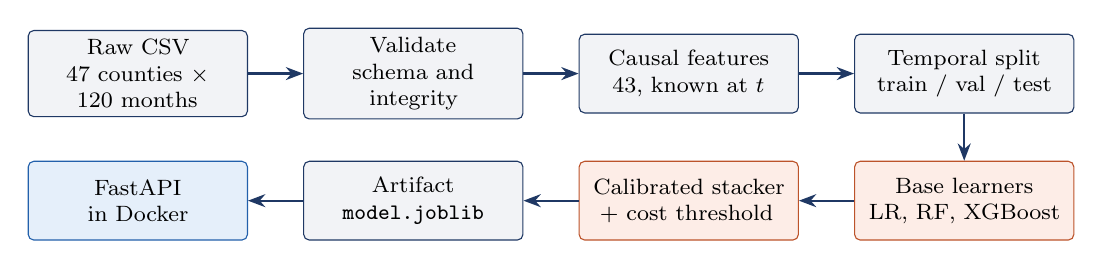
\begin{tikzpicture}[
  box/.style={draw=navy,fill=navy!6,rounded corners=2pt,minimum height=10mm,text width=2.55cm,align=center,font=\footnotesize},
  arr/.style={-{Stealth[length=2.2mm]},thick,navy},
  node distance=6mm and 7mm]
  \node[box] (a) {Raw CSV\\47 counties $\times$ 120 months};
  \node[box,right=of a] (b) {Validate\\schema and integrity};
  \node[box,right=of b] (c) {Causal features\\43, known at $t$};
  \node[box,right=of c] (d) {Temporal split\\train / val / test};
  \node[box,below=of d,fill=ora!12,draw=ora!80!black] (e) {Base learners\\LR, RF, XGBoost};
  \node[box,left=of e,fill=ora!12,draw=ora!80!black] (f) {Calibrated stacker\\+ cost threshold};
  \node[box,left=of f] (g) {Artifact\\\code{model.joblib}};
  \node[box,left=of g,fill=blu!12,draw=blu!80!black] (h) {FastAPI\\in Docker};
  \draw[arr] (a)--(b); \draw[arr] (b)--(c); \draw[arr] (c)--(d); \draw[arr] (d)--(e);
  \draw[arr] (e)--(f); \draw[arr] (f)--(g); \draw[arr] (g)--(h);
\end{tikzpicture}
\caption{Pipeline architecture. Base learners are fitted on the training period; the stacker and threshold on the validation period.}
\end{figure}

\begin{itemize}
  \item \textbf{Validation} (\code{data.py}) fails hard on missing columns, duplicate keys, impossible values and unknown categories.
  \item \textbf{Features} (43) use data up to month $t$ only: escalation lags and 3/6/12-month rolling shares, rolling indicator means, same-region and national escalation shares (a spill-over proxy), empirical-Bayes Markov transition probabilities, calendar terms and one-hot categories.
  \item \textbf{Empirical-Bayes Markov feature.} For county $c$ in state $s\in\{0,1\}$ (not escalating / escalating) the probability of escalating next month is estimated from the transitions observed up to $t$ and shrunk toward the pooled rate:
  \begin{equation}
     \hat p_{c,s,t}=\frac{n^{\to 1}_{c,s,t}+k\,\bar p_{s,t}}{n_{c,s,t}+k},\qquad k=10 .
  \end{equation}
  \item \textbf{Leakage guard.} \code{tests/test\_features.py} corrupts every observation after a cut-off month and asserts that no feature at or before the cut-off changes (cf.\ \cite{kaufman2012}). The test was shown to be sensitive by planting two deliberately leaky features; it flagged both and left the real features alone.
\end{itemize}

% ------------------------------------------------------------------ 4
\section{Technique choices, and what was left out}
\subsection*{Used, and why}
\begin{longtable}{@{}>{\raggedright\arraybackslash}p{3.7cm}>{\raggedright\arraybackslash}p{11.9cm}@{}}
\toprule
\textbf{Technique} & \textbf{Why it fits} \\
\midrule
\endhead
Logistic regression & Interpretable baseline that the proposal asks for. It receives the largest weight in the blend (0.48 on the logit scale). \\
Random forest~\cite{breiman2001} & Captures non-linear interactions and region effects at low tuning cost. \\
XGBoost~\cite{chen2016} & Strong on structured tabular data; handles feature interactions. \\
Calibrated logistic stacker~\cite{wolpert1992,platt1999} & Combines the three learners on the validation period and doubles as a Platt-style calibrator, so outputs are usable probabilities. \\
Cost-sensitive threshold & The decision rule reflects unequal error costs. \\
County-block bootstrap & Rows within a county are autocorrelated, so whole counties are resampled to avoid over-confident intervals. \\
Permutation importance & Model-agnostic importance computed on the validation set, so the test set stays untouched. \\
PSI drift check & Quantifies the shift between periods. \\
MLflow tracking and registry & Records every run's parameters, validation and test metrics, tables and model, with the three base learners as nested runs for side-by-side comparison. A passing model is registered as \code{stbmse-ensemble} with alias \code{production}. \\
Quality gate (validation only) & The best base learner must beat persistence by at least 0.05 PR-AUC on validation, scores must be finite and the alert threshold non-degenerate. A failed gate exits non-zero, writes no model and registers nothing. It uses validation data only, so the test period stays untouched by any decision. \\
GitHub Actions CI/CD & CI on every push: train with the gate, audits, drift report, tests, Docker build, then run the container and call it. CD (push to the container registry) only from the default branch and only if CI passed. \\
Evidently AI drift report & Course-standard drift detection on inputs, predictions and target between the training and test periods (Section~\ref{sec:drift}). \\
\bottomrule
\end{longtable}

\subsection*{Considered and not used}
\begin{longtable}{@{}>{\raggedright\arraybackslash}p{3.7cm}>{\raggedright\arraybackslash}p{11.9cm}@{}}
\toprule
\textbf{Technique} & \textbf{Reason} \\
\midrule
\endhead
LSTM / GRU / Transformer & 47 series of 120 points (about 5{,}600 rows) is too little data for sequence models to beat engineered lags and boosted trees, and interpretability would suffer. This is an argued position, not a tested one. \\
SVM & Needs scaling and a separate probability-calibration step, with no expected gain over the three learners already used. \\
LightGBM & Redundant with XGBoost on a dataset this small. \\
K-Means, DBSCAN, PCA, t-SNE & The task is supervised and a label exists. Clustering counties could describe regions but would not improve a one-month-ahead forecast. \\
LLM fine-tuning, RAG, agents & There is no text in the file; adding an LLM would be a gimmick. \\
SHAP & Not installed in the environment; permutation importance was used instead. SHAP is the natural next step for per-prediction explanations. \\
Hyperparameter search & Hyperparameters were fixed, not tuned (no Optuna or grid search). This is a limitation, not a considered exclusion. \\
\bottomrule
\end{longtable}

% ------------------------------------------------------------------ 5
\section{Results}\label{sec:results}
All figures are for the 2022--2024 test period ($n=1{,}692$ county-months) with 95\% county-block bootstrap confidence
intervals (500 resamples). PR-AUC is emphasised because it is more informative than ROC-AUC when positives are a minority~\cite{saito2015}; here the no-skill PR-AUC equals the test base rate, 0.43.

\begin{table}[!htbp]
\centering\footnotesize
\setlength{\tabcolsep}{4.5pt}
\caption{Test-period performance. Recall and false-alarm rate use each model's own validation-tuned threshold.}
\label{tab:results}
\begin{tabular}{@{}lcccrr@{}}
\toprule
\textbf{Model} & \textbf{PR-AUC (95\% CI)} & \textbf{ROC-AUC (95\% CI)} & \textbf{Recall} & \textbf{False-alarm} & \textbf{Brier} \\
\midrule
Persistence baseline & 0.498 (0.433--0.559) & 0.609 (0.571--0.644) & 0.55 & 0.34 & 0.383 \\
Logistic regression & 0.594 (0.507--0.679) & 0.672 (0.623--0.715) & 0.97 & 0.89 & 0.227 \\
Random forest & \textbf{0.619} (0.533--0.692) & \textbf{0.700} (0.644--0.743) & 0.93 & 0.75 & 0.221 \\
XGBoost & 0.587 (0.512--0.660) & 0.678 (0.623--0.719) & 0.89 & 0.72 & 0.231 \\
\textbf{ST-BMSE ensemble} & 0.608 (0.520--0.689) & 0.691 (0.639--0.734) & 0.94 & 0.81 & 0.221 \\
\bottomrule
\end{tabular}
\end{table}

\begin{figure}[!htbp]
  \centering
  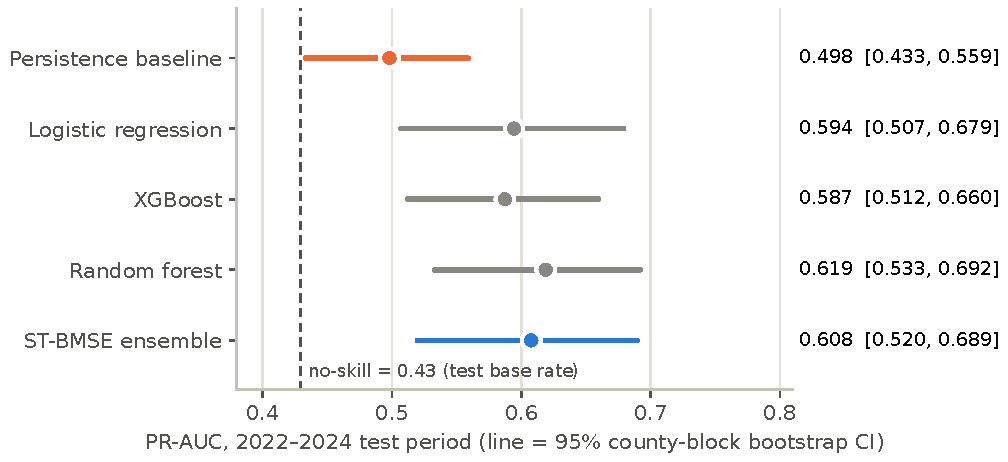
\includegraphics[width=0.97\linewidth]{figures/fig_results.pdf}
  \caption{PR-AUC on the test period with 95\% county-block bootstrap intervals. Only the ensemble's gain over persistence is clearly outside noise.}
  \label{fig:results}
\end{figure}

\begin{table}[!htbp]
\centering\small
\caption{Paired differences in PR-AUC, on the same resampled counties.}
\begin{tabularx}{\linewidth}{@{}lccX@{}}
\toprule
\textbf{Comparison} & \textbf{Difference} & \textbf{95\% CI} & \textbf{Reading} \\
\midrule
Ensemble $-$ persistence & $+0.109$ & $0.062$ to $0.161$ & Real improvement \\
Ensemble $-$ random forest & $-0.011$ & $-0.031$ to $+0.016$ & No evidence the ensemble beats a single random forest \\
Ensemble $-$ logistic regression & $+0.013$ & $0.002$ to $0.026$ & Small gain, borderline \\
\bottomrule
\end{tabularx}
\end{table}

\Needspace{8\baselineskip}
\textbf{Interpretation, stated plainly.}
\begin{itemize}
  \item The model forecasts better than persistence, and the gap lies outside bootstrap noise. That is the baseline the proposal names.
  \item Stacking did not help over the best single learner. The proposal's central claim, that the ensemble is better because it combines complementary learners, is \textbf{not supported} on this data.
  \item ROC-AUC of about 0.69 means moderate discrimination, not strong. The forecasting signal is modest.
  \item Calibration is acceptable (expected calibration error 0.049; Figure~\ref{fig:cal}). Probabilities are slightly too low in the lower bins because the test base rate exceeds the training one.
  \item \textbf{The tuned alert is operationally poor.} The threshold (0.18) was chosen on 2020--2021, when 24\% of months escalated. In the 43\% test regime it flags most counties: recall 0.94 but a false-alarm rate of 0.81. For December 2024, \textbf{46 of 47 counties alert} at 0.18 and 8 of 47 at 0.50. The API therefore exposes a \code{threshold} override; the right value should be set with practitioners, not by an assumed cost ratio.
  \item Most important inputs on the validation period (permutation importance): the 3-month mean social-unrest score, the 6- and 12-month escalation shares, cumulative county history, the Markov ``enter escalation'' probability and the North Eastern region indicator.
\end{itemize}

\begin{figure}[!htbp]
  \centering
  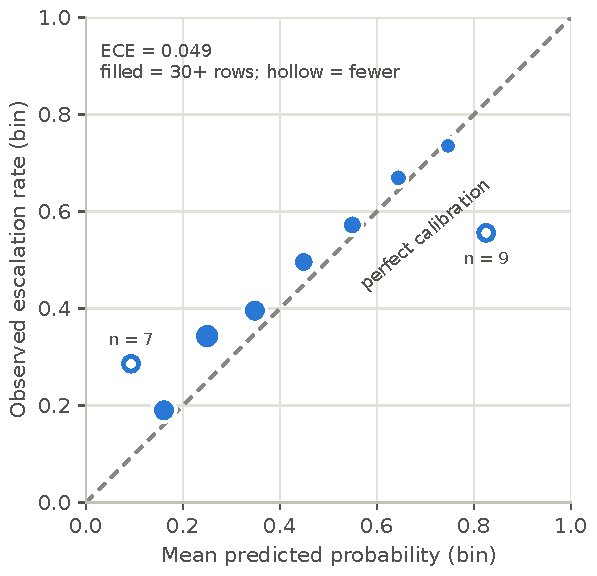
\includegraphics[width=0.55\linewidth]{figures/fig_calibration.pdf}
  \caption{Reliability diagram on the test period. Points near the diagonal are well calibrated; the two hollow points rest on 7 and 9 rows and should not be over-read.}
  \label{fig:cal}
\end{figure}

% ------------------------------------------------------------------ 6
\section{Audits}
\subsection{Leakage audit}\label{sec:leak}
Figure~\ref{fig:leak} compares a nowcast with honest forecasts. Same-month indicators almost determine the same-month
label: \code{Sentiments} alone gives 0\% escalation for Positive and Neutral rows and 83\% for Negative rows. A random split on this file would
report a near-perfect model.

\begin{figure}[!htbp]
  \centering
  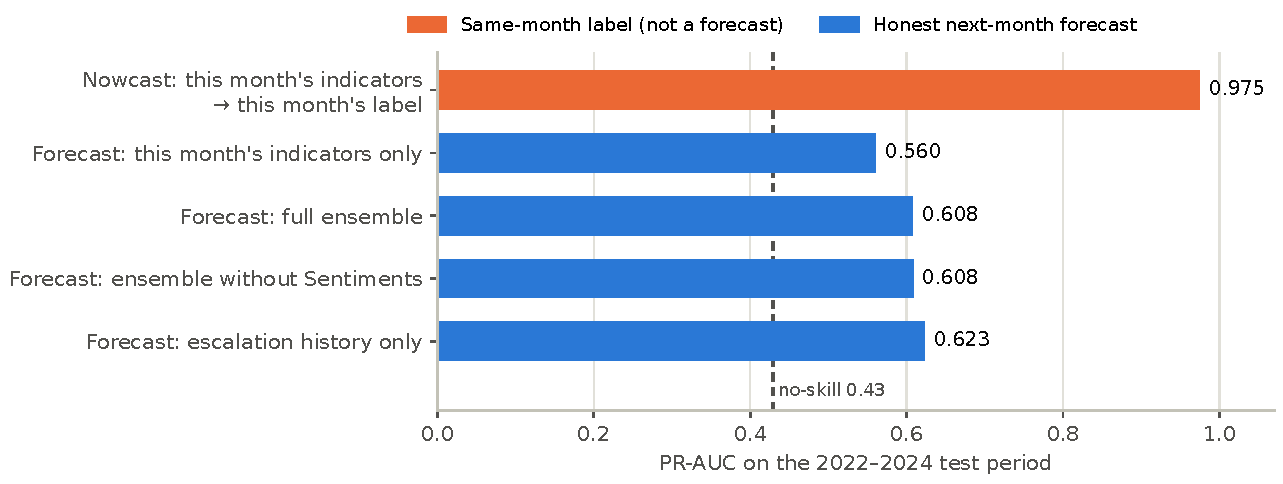
\includegraphics[width=0.97\linewidth]{figures/fig_leakage.pdf}
  \caption{PR-AUC for a same-month nowcast versus next-month forecasts. For the honest task, the indicator columns add nothing measurable beyond escalation history.}
  \label{fig:leak}
\end{figure}

For the honest next-month task the history-only ensemble (0.623) scores as well as, or slightly higher than, the full one (0.608).
The socio-economic indicators are therefore not demonstrated to help forecasting.

\subsection{Drift}\label{sec:drift}
The escalation rate rises from 20\% to 24\% to 43\% across the training, validation and test periods (Figure~\ref{fig:drift}). Two independent checks agree on the direction.

\textbf{Evidently AI} compares the training period (2{,}679 rows) with the test period (1{,}692 rows) using its default tests: normed Wasserstein distance for numbers and Jensen--Shannon distance for categories, both with threshold 0.1.
\begin{itemize}
  \item \textbf{27 of 32 columns (84\%) drifted}, and dataset-level drift is detected.
  \item \textbf{Prediction drift:} the model's own predicted probability drifted strongly (score 1.31 against a 0.1 threshold), and \textbf{target drift} was flagged too (0.17).
  \item Largest input shifts: the national and regional spill-over shares (2.65 and 1.08), and the social-unrest score and its lags (1.2 to 1.7).
  \item \textbf{Stable:} \code{Region}, \code{Security\_Force\_Response\_Time} with its lag, and the calendar terms. The calendar terms act as a built-in sanity check: month of year should not drift, and it does not.
\end{itemize}
The hand-built \textbf{population stability index (PSI)} check found 18 continuous features above 0.25, the usual ``major shift'' line. PSI on rate-like and discrete features is inflated by
coarse bins, so it is a direction rather than a magnitude. Evidently reports that the inputs moved, not that the model got worse; accuracy on the test period (Section~\ref{sec:results}) is the measure of that.
Practical implication: the model must be retrained and the threshold re-tuned on recent data.

\subsection{Per-region performance}
At the tuned threshold the false-alarm burden is uneven (Figure~\ref{fig:region}). Northern and North Eastern regions have a false-alarm
rate of 1.00 (every quiet month flagged), Coastal 0.94 and Nyanza 0.90, against 0.64--0.65 for Eastern and Western. PR-AUC ranges from 0.47 (Coastal) to 0.76 (Central).
Regions contain only 3 to 11 counties, so these differences are indicative, not conclusive. Equal thresholds do not give equal treatment.

\begin{figure}[!htbp]
  \centering
  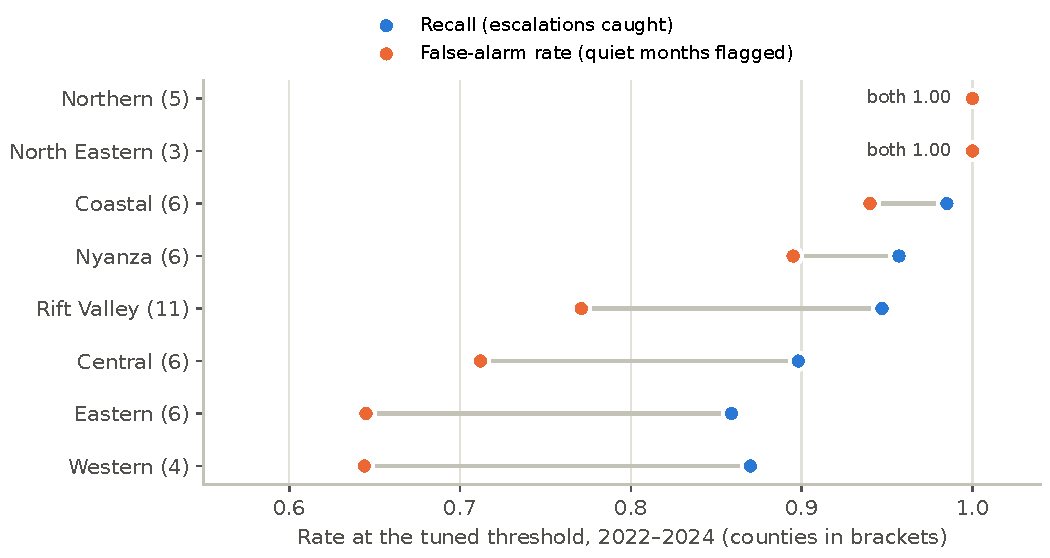
\includegraphics[width=0.97\linewidth]{figures/fig_region.pdf}
  \caption{Recall and false-alarm rate per region at the tuned threshold, test period.}
  \label{fig:region}
\end{figure}

% ------------------------------------------------------------------ 7
\section{Gap between the proposal and what was delivered}
\begin{longtable}{@{}>{\raggedright\arraybackslash}p{5.6cm}>{\raggedright\arraybackslash}p{10.0cm}@{}}
\toprule
\textbf{Proposal} & \textbf{Delivered} \\
\midrule
\endhead
ACLED events and KNBS indicators & Synthetic county-month data built to the proposal's design (no real event counts, fatalities or KNBS series); real ACLED and KNBS data is the planned next stage. \\
Spatial spill-over from neighbouring counties & Same-region share as a proxy (no adjacency data). \\
Data-quality challenges (missing events, reporting changes, geocoding errors) & Not present: synthetic data are complete by construction, so the validation stage is built and tested but real-world messiness is not exercised. \\
Class imbalance because escalation is rare & Escalation is common here (28\% overall, 43\% in test). \\
Stacked ensemble expected to outperform & Not shown; it ties a single random forest. \\
Human-in-the-loop prototype in the ThreatGuard AI dashboard & A prediction API with context fields for an analyst; not integrated with the dashboard. \\
\bottomrule
\end{longtable}

\medskip
To use real data: obtain ACLED and KNBS, aggregate to county-month, define ``escalation'' explicitly (the proposal does not), and map the result to
the schema in \code{config.REQUIRED\_COLUMNS} or extend \code{data.py}.

% ------------------------------------------------------------------ 8
\section{Deployment and real-world relevance}
A FastAPI service (\code{/predict}, \code{/predict/batch}, \code{/health}, \code{/model-info}) loads the serialised artifact. Features are rebuilt at
serving time with the same code as training, so training and serving cannot diverge. The API returns the probability, the base-model probabilities and the context an
analyst needs (recent escalation share, region peers, Markov probability). It was tested with pytest (32 tests passing) and with live HTTP calls.

\textbf{Frontend.} The API serves a single-page analyst view at \code{/ui} (Figure~\ref{fig:ui}): all 47 counties ranked by predicted probability, an as-of month selector, an alert-threshold slider,
region and alerts-only filters, and a detail panel showing what each of the three models says plus context an analyst can check. When the threshold makes nearly every county alert (as the tuned 0.18 does)
the page says so and advises raising it. It is a real client of the JSON endpoints, makes no external requests, inserts API values as text only, and these properties are covered by tests.
It was checked in headless Edge at desktop and phone widths in light and dark mode, and served from the Docker container; it has not been tested in Firefox or Safari, or with a screen reader.

\begin{figure}[!htbp]
  \centering
  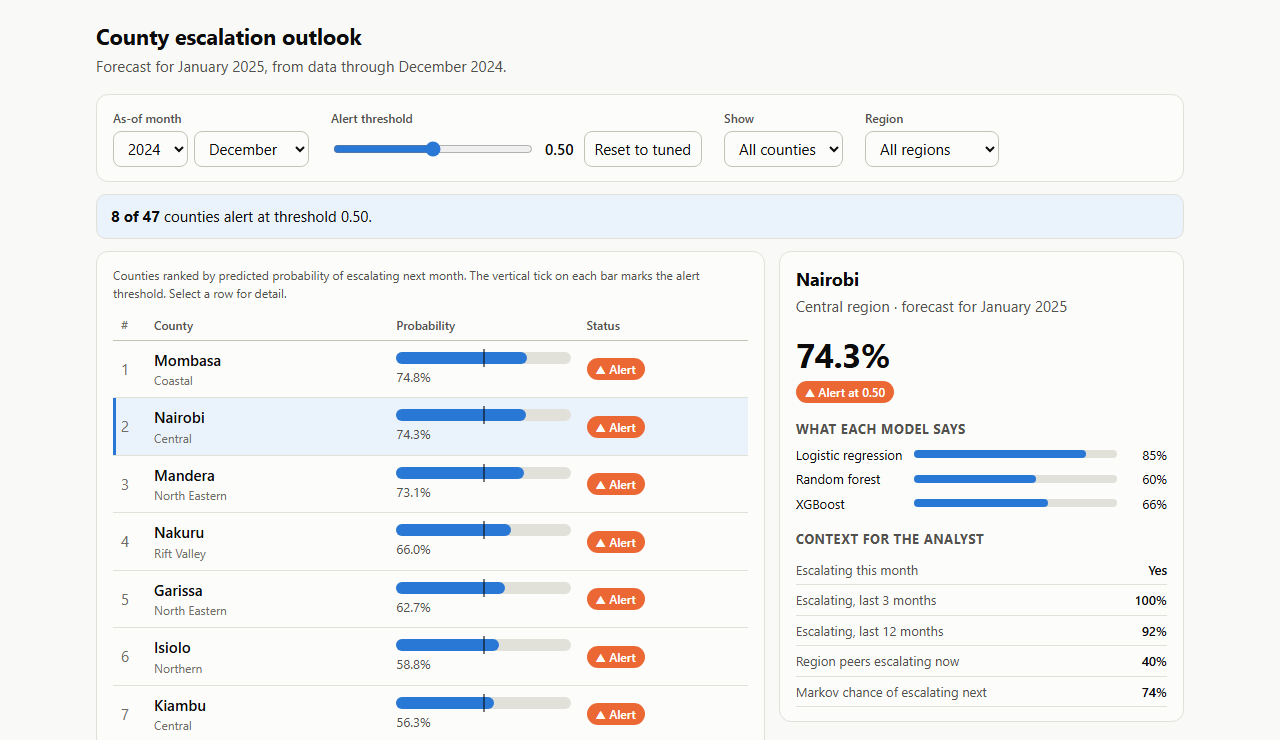
\includegraphics[width=0.97\linewidth]{figures/ui_screenshot.png}
  \caption{The analyst view served at \code{/ui}, here with the threshold raised to 0.50 so that 8 of 47 counties alert and the ranking is informative. The tick on each bar marks the threshold.}
  \label{fig:ui}
\end{figure}

\textbf{Experiment tracking and the quality gate.} Every training run is logged to MLflow: parameters, validation and test metrics, tables, the model, and one nested run per base learner. The gate runs on
\emph{validation data only}. A failed gate exits with code 1, writes no model artifact and registers nothing; the failed run is still logged and tagged \code{quality\_gate=failed}. This was exercised in both directions.
On the real data the gate passes (the best base learner beats persistence by $+0.179$ PR-AUC on validation, against a required $+0.05$). Demanding an impossible $+0.90$ stopped the pipeline with exit code 1,
left the model file untouched and left the registry holding only the passing version. The registered model loads back from \code{models:/stbmse-ensemble@production}.

\textbf{CI/CD.} \code{.github/workflows/ci.yml} runs on every push and pull request: install, train with the gate, audits and Evidently report, pytest, Docker build, then run the container and call
\code{/health}, \code{/predict} and an invalid request, which must return HTTP 422. Publishing to the GitHub Container Registry happens only on the default branch and only if CI passed.
\textbf{The workflow ran green on GitHub on its first push} (run 44397520310): both the \code{ci} job and the \code{cd} job (build and push to the container registry) succeeded.
Not verified: the published image could not be listed independently (the available token lacks the \code{read:packages} scope), the workflow file was not checked with a dedicated linter such as \code{actionlint}, and the gate's blocking behaviour was proven locally rather than on GitHub.

\textbf{Container verification.} The Docker image was rebuilt from the slimmed serving requirements (no MLflow, Evidently or test tools in the image) and run exactly as the CI job does (Docker Desktop, Windows~11).
The quality gate runs during \code{docker build}, so a failing gate would fail the build. The image is 1.3~GB; about 200~MB of that is a GPU-communication library that XGBoost's Linux wheel pulls in and this CPU-only service does not use.
The container passed its health check, runs as a non-root user and served
correct predictions and validation errors over HTTP. The model trained inside the Linux image differs slightly from the Windows-trained one used for the tables above (XGBoost is not bit-identical across
platforms): ensemble PR-AUC 0.609 vs.\ 0.608, but tuned threshold 0.16 vs.\ 0.18 and false-alarm rate 0.89 vs.\ 0.81. Rankings and conclusions are unchanged; alert-level figures are not exactly reproducible across operating systems.

% ------------------------------------------------------------------ 9
\section{Limitations}
\begin{itemize}
  \item The data are synthetic: results demonstrate the method and say nothing about real conflict in Kenya.
  \item Synthetic data are clean and complete by construction, so raw-data problems (missing or duplicated events, geocoding errors) are not exercised; the evaluation's realism comes from the temporal protocol and the data's own prior shift.
  \item One train/validation/test split; no rolling-origin evaluation.
  \item Hyperparameters were fixed and not tuned.
  \item The CI/CD workflow ran once on GitHub; the published image was not independently inspected, the file was not linted, and the gate's blocking behaviour was proven locally, not on GitHub.
  \item The quality-gate margin ($+0.05$ PR-AUC over persistence) is a judgement, not derived from a requirement.
  \item The 5:1 cost ratio is assumed.
  \item The alert threshold does not transfer across regimes; recalibrate on recent data.
  \item Spill-over is a regional proxy, not geographic adjacency.
  \item No causal claim: importance scores show predictive association only.
\end{itemize}

% ------------------------------------------------------------------ 10
\section{Reproduce}
\begin{lstlisting}
python -m pip install -r requirements.txt
python run_pipeline.py            # gate + MLflow + Evidently; exits 1 if the gate fails
python -m pytest -q
mlflow ui --backend-store-uri sqlite:///mlflow.db   # browse runs and the model registry
python latex/make_figures.py      # regenerates the figures in this report
\end{lstlisting}
The Evidently report is written to \code{reports/evidently\_drift\_report.html}; open it in a browser.

% ------------------------------------------------------------------ refs
\begin{thebibliography}{9}\small
\bibitem{raleigh2010} C.~Raleigh, A.~Linke, H.~Hegre and J.~Karlsen. Introducing ACLED: An Armed Conflict Location and Event Dataset. \emph{Journal of Peace Research}, 47(5):651--660, 2010.
\bibitem{kaufman2012} S.~Kaufman, S.~Rosset, C.~Perlich and O.~Stitelman. Leakage in data mining: Formulation, detection, and avoidance. \emph{ACM Transactions on Knowledge Discovery from Data}, 6(4), 2012.
\bibitem{breiman2001} L.~Breiman. Random forests. \emph{Machine Learning}, 45(1):5--32, 2001.
\bibitem{chen2016} T.~Chen and C.~Guestrin. XGBoost: A scalable tree boosting system. In \emph{Proc.\ 22nd ACM SIGKDD}, pages 785--794, 2016.
\bibitem{wolpert1992} D.~H.~Wolpert. Stacked generalization. \emph{Neural Networks}, 5(2):241--259, 1992.
\bibitem{platt1999} J.~Platt. Probabilistic outputs for support vector machines and comparisons to regularized likelihood methods. In \emph{Advances in Large Margin Classifiers}, pages 61--74. MIT Press, 1999.
\bibitem{saito2015} T.~Saito and M.~Rehmsmeier. The precision-recall plot is more informative than the ROC plot when evaluating binary classifiers on imbalanced datasets. \emph{PLoS ONE}, 10(3):e0118432, 2015.
\bibitem{serrano2026} J.~Serrano and E.~L.~Bundi. \emph{Applied Machine Learning: From Foundations to Production Systems}. iLabAfrica, Strathmore University, 2026 (course textbook).
\end{thebibliography}

\end{document}
